\chapter{ゲーム理論}

この章では、ランダムな要素を含まない2人用ゲームに焦点を当てます。
そして相手が何をやってもゲームに勝てるような戦略(もしそのような戦略)を見つけることです。
このようなゲームには一般的な戦略があることがわかり、Nimを使ってゲームを分析することができます。
まず、プレイヤーが山から棒を取り除く簡単なゲームを分析し、その後に一般化を行います。

\section{ゲームの状態 - Game states}

最初に$n$本の棒があるゲームを考えます。
プレイヤー$A$と$B$は交互に交代します。最初はプレイヤーAからスタートします。
各手番で1本、2本、3本の棒を山から取り除き、最後の棒を取り除いたプレーヤーがゲームに勝つとします。
n=10の場合、次のようにゲームを進めることができます。

For example, if $n=10$, the game may proceed as follows:
\begin{itemize}[noitemsep]
\item プレイヤーAは2本取る(残り8本)
\item プレイヤーBは3本取る(残り5本)
\item プレイヤーAは1本取る(残り4本)
\item プレイヤーBは2本取る(残り2本)
\item プレイヤーAは2本取って勝ち
\end{itemize}

このゲームは$0,1,2,\ldots,n$の状態からなり、
状態の数は残っているスティックの数に対応します。

\subsubsection{勝ち状態と負け状態 - Winning and losing states}

\index{勝ち状態 - winning state}
\index{負け状態 - losing state}

\key{勝利状態} とは適切に動けば必ず勝ちが確定する状態です。
\key{敗北状態} とは相手が最適なプレイをすればゲームに負ける状態である。
このように、ゲームの状態をすべて分類することで、それぞれの状態が「勝ちの状態」と「負けの状態」のどちらかになることがわかります。

上のゲームを考えます。
状態0は明らかに負け状態で、プレイヤーは何も手を打てません。
状態1、2、3は、最後の1つを取れるので勝ちの状態です。
状態4は逆にどの手を打っても相手が勝ち状態になるため、負け状態と言えます。
一般的には、現在の状態から負け状態にできる現在の状態は勝ち状態であり、
そうでなければ、現在の状態は負け状態である。
これを を利用して、可能な手がない負け状態から始まるゲームのすべての状態を分類 することができます。

状態 $0 \ldots 15$を分類します(Wは勝ち状態、Lは負け状態)。

\begin{center}
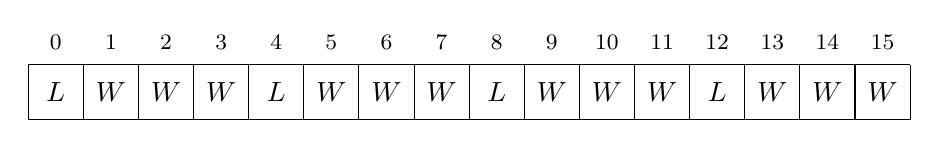
\begin{tikzpicture}[scale=0.7]
\draw (0,0) grid (16,1);

\node at (0.5,0.5) {$L$};
\node at (1.5,0.5) {$W$};
\node at (2.5,0.5) {$W$};
\node at (3.5,0.5) {$W$};
\node at (4.5,0.5) {$L$};
\node at (5.5,0.5) {$W$};
\node at (6.5,0.5) {$W$};
\node at (7.5,0.5) {$W$};
\node at (8.5,0.5) {$L$};
\node at (9.5,0.5) {$W$};
\node at (10.5,0.5) {$W$};
\node at (11.5,0.5) {$W$};
\node at (12.5,0.5) {$L$};
\node at (13.5,0.5) {$W$};
\node at (14.5,0.5) {$W$};
\node at (15.5,0.5) {$W$};

\footnotesize
\node at (0.5,1.4) {$0$};
\node at (1.5,1.4) {$1$};
\node at (2.5,1.4) {$2$};
\node at (3.5,1.4) {$3$};
\node at (4.5,1.4) {$4$};
\node at (5.5,1.4) {$5$};
\node at (6.5,1.4) {$6$};
\node at (7.5,1.4) {$7$};
\node at (8.5,1.4) {$8$};
\node at (9.5,1.4) {$9$};
\node at (10.5,1.4) {$10$};
\node at (11.5,1.4) {$11$};
\node at (12.5,1.4) {$12$};
\node at (13.5,1.4) {$13$};
\node at (14.5,1.4) {$14$};
\node at (15.5,1.4) {$15$};
\end{tikzpicture}
\end{center}

このゲームは簡単で、
$k$が4で割り切れる場合は負け。それ以外は勝ち状態です。
このゲームの最適なプレイ方法は、スティックが4で割り切れる状態にすれば良いです。
もちろん、こちらが動くときに棒の数が4で割り切れないことが条件です。
もし4で割り切れるなら、相手が最適な手を打つ限り勝てません。

\subsubsection{状態グラフ - State graph}

ここで,別のゲームを考えます。
各状態 $k$ において,$x$ が $k$ より小さく $k$ を割り切れる $x$ 本の棒を取り除けるとします。
例えば,状態8では1本,2本,4本の棒を取り除くことができるが、状態7では1本の棒を取り除くことだけが許されるとします。


次の図は、状態$1 \ldots 9$を状態グラフで表したもので、ノードが状態、エッジが取りうる移動です。

\begin{center}
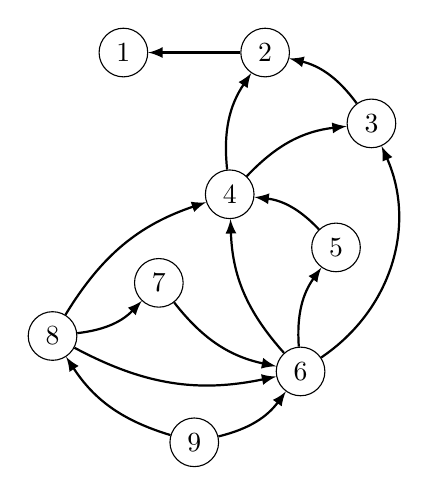
\begin{tikzpicture}[scale=0.9]
\node[draw, circle] (1) at (0,0) {$1$};
\node[draw, circle] (2) at (2,0) {$2$};
\node[draw, circle] (3) at (3.5,-1) {$3$};
\node[draw, circle] (4) at (1.5,-2) {$4$};
\node[draw, circle] (5) at (3,-2.75) {$5$};
\node[draw, circle] (6) at (2.5,-4.5) {$6$};
\node[draw, circle] (7) at (0.5,-3.25) {$7$};
\node[draw, circle] (8) at (-1,-4) {$8$};
\node[draw, circle] (9) at (1,-5.5) {$9$};

\path[draw,thick,->,>=latex] (2) -- (1);
\path[draw,thick,->,>=latex] (3) edge [bend right=20] (2);
\path[draw,thick,->,>=latex] (4) edge [bend left=20] (2);
\path[draw,thick,->,>=latex] (4) edge [bend left=20] (3);
\path[draw,thick,->,>=latex] (5) edge [bend right=20] (4);
\path[draw,thick,->,>=latex] (6) edge [bend left=20] (5);
\path[draw,thick,->,>=latex] (6) edge [bend left=20] (4);
\path[draw,thick,->,>=latex] (6) edge [bend right=40] (3);
\path[draw,thick,->,>=latex] (7) edge [bend right=20] (6);
\path[draw,thick,->,>=latex] (8) edge [bend right=20] (7);
\path[draw,thick,->,>=latex] (8) edge [bend right=20] (6);
\path[draw,thick,->,>=latex] (8) edge [bend left=20] (4);
\path[draw,thick,->,>=latex] (9) edge [bend left=20] (8);
\path[draw,thick,->,>=latex] (9) edge [bend right=20] (6);
\end{tikzpicture}
\end{center}

このゲームの最終状態は常に状態1で、
有効な手がないため負け状態です。
状態$1 \ldots 9$の勝ち状態と負け状態は次のとおりです。

\begin{center}
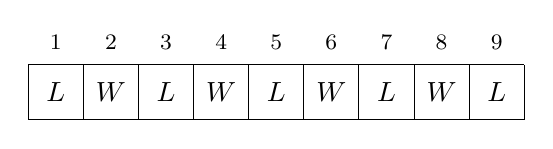
\begin{tikzpicture}[scale=0.7]
\draw (1,0) grid (10,1);

\node at (1.5,0.5) {$L$};
\node at (2.5,0.5) {$W$};
\node at (3.5,0.5) {$L$};
\node at (4.5,0.5) {$W$};
\node at (5.5,0.5) {$L$};
\node at (6.5,0.5) {$W$};
\node at (7.5,0.5) {$L$};
\node at (8.5,0.5) {$W$};
\node at (9.5,0.5) {$L$};

\footnotesize
\node at (1.5,1.4) {$1$};
\node at (2.5,1.4) {$2$};
\node at (3.5,1.4) {$3$};
\node at (4.5,1.4) {$4$};
\node at (5.5,1.4) {$5$};
\node at (6.5,1.4) {$6$};
\node at (7.5,1.4) {$7$};
\node at (8.5,1.4) {$8$};
\node at (9.5,1.4) {$9$};
\end{tikzpicture}
\end{center}

意外かもしれませんがこのゲームは、偶数の時勝ち状態で、奇数の時負け状態です。

\section{Nim - Nim game}

\index{Nim - nim game}

\key{Nim - nim game}は単純なゲームですが同じ戦略を用いて他の多くのゲームを行 うことができるため、
ゲーム理論において重要な考え方です。

nimには$n$個の山があり、各山にはある数の棒があります。
プレイヤーは交互に移動し、まだ棒が入っている山を選び、そこから 任意の本数の棒を取り除きます。
最後のスティックを取り除いたプレイヤーが勝者です。

nimの初期状態は$[x_1,x_2,\ldots,x_n]$で与えられ、
$x_k$ は$k$個目の山のスティックの数とします。
例えば,$[10, 12, 5]$ は10,12,5のスティックを持つ三つの山がある初期状態です。
$[0,0,\ldots,0]$の状態は,棒を1本も取り出せないので負け状態であり,これが常に最終状態です。

\subsubsection{考察 - Analysis}

\index{nim sum}
nim sum $s$を用いて分析を行うことができます\footnote{The optimal strategy
for nim was published in 1901 by C. L. Bouton \cite{bou01}.}。
$s = x_1 \oplus x_2 \oplus \cdots \oplus x_n$として$\oplus$はXOR演算です。
$s$が0の時は負けでそれ以外は勝ち状態です。
例えば$[10,12,5]$は$10 \oplus 12 \oplus 5 = 3$なので勝ち状態です。

ですがnim sumとnimゲームはどのように関係しているのでしょうか?
nimの状態が変化したときに、nim sumがどのように変化するかを見ていいます。
最終状態 $[0,0,\ldots,0]$ は負け状態で、その$s$は0です。
他の負け状態を考えるとどのような動きも勝ち状態になります。
なぜなら、一つの値$x_k$が変化すると、nim sumも変化するので、どんな作業の後もnim sumは0と異なるからです。

勝ち組の状態を考えます。$x_k \oplus s < x_k$となる山$k$があれば,負け状態に遷移できます。つまり勝てます。
この場合,山$k$からスティックを取り除き,$x_k \oplus s$のスティックを含むようにすれば,負け状態に移行できます。
このような山は必ず存在し、いずれかの$x_k$ は s の 左端の1ビットの1ビットを持った数です。

$[10, 12, 5]$の状態を考えてみましょう。
この状態はnim sumが3なので勝ちの状態であり、そのような 手を見つけます。

\begin{center}
\begin{tabular}{r|r}
10 & \texttt{1010} \\
12 & \texttt{1100} \\
5 & \texttt{0101} \\
\hline
3 & \texttt{0011} \\
\end{tabular}
\end{center}

この場合、10本ある山がnim sumの左端の1ビットの位置に1ビットを持つ唯一の山です。

\begin{center}
\begin{tabular}{r|r}
10 & \texttt{10\underline{1}0} \\
12 & \texttt{1100} \\
5 & \texttt{0101} \\
\hline
3 & \texttt{00\underline{1}1} \\
\end{tabular}
\end{center}

山の本数は $10 \oplus 3 = 9$にしたいので1本だけ取ります。
この後、状態は$[9, 12, 5]$となり、負け状態に遷移できます。

\begin{center}
\begin{tabular}{r|r}
9 & \texttt{1001} \\
12 & \texttt{1100} \\
5 & \texttt{0101} \\
\hline
0 & \texttt{0000} \\
\end{tabular}
\end{center}

\subsubsection{misere nim game - Misère game}

\index{misère game}

\key{misere nim game - misère game}はゲームの目的が逆です。
つまり、最後のスティックを取ったプレイヤーがゲームに負けます。
misere nim gameは標準のnimとほぼ同じ様に考えられます。

最初は標準的なnimゲームのようを行うが、ゲームの終盤に戦略を変えます。
戦略を変えるのは、次の手の後に各山が最大で1本の棒を含むような状況で導入されることになる。

オリジナルのゲームでは、1本の棒を持つヒープが偶数個になるような手を選ぶべきです。
しかし、misèreゲームでは、1本の棒で奇数個の山ができるようにします。

まず、この戦略が変化する状態が必ずゲームに現れます。
この状態になったとき、ちょうど複数のスティックを持つ山が一つ含まれているので、
ニムサムは0ではないので、勝利が確定します。

\section{スプレイグ・グランディの定理 - Sprague–Grundy theorem}

\index{スプレイグ・グランディの定理 - Sprague–Grundy theorem}

\key{スプレイグ・グランディの定理 - Sprague–Grundy theorem}\footnote{The theorem was
independently discovered by R. Sprague \cite{spr35} and P. M. Grundy \cite{gru39}.}
により、nimで用いられている戦略は、以下の要件を満たすべてのゲームに一般化できます。

\begin{itemize}[noitemsep]
\item 2人のプレイヤーが交互にプレイする
\item ゲームは状態から構成される。ある状態において可能な手は誰の手番であるかには依存しないこと。
\item プレイヤーが手を出せなくなるとゲーム終了となる
\item ゲームは遅かれ早かれ必ず終わります。
\item プレイヤーは状態と許容される手について完全な情報を持っており、ゲームにランダム性はない。
\end{itemize}
このアイデアは、各ゲーム状態のグランディ数をnim山に紐づけて管理することにあります。
すべての状態のグランディ数が分かれば、nimゲームのようにプレイができます。

\subsubsection{Grundy数 - Grundy numbers}

\index{Grundy数 - Grundy number}
\index{MEX - mex function}

ゲームの状態の\key{Grundy数 - Grundy number}とは次のように示されます。
\[\textrm{mex}(\{g_1,g_2,\ldots,g_n\}),\]
ここで、$g_1,g_2,\ldots,g_n$
は移動可能な状態のGrundy数で、mex関数はその集合に含まれない最小の非負の数のことです。
例えば、$\textrm{mex}(\{0,1,3\})=2$です。
ある状態で移動可能なものがない場合、$\textrm{mex}(\emptyset)=0$.
なので、そのグランディ数は0とします。

例えば、以下を考えます。
\begin{center}
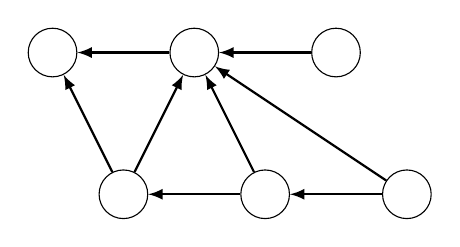
\begin{tikzpicture}[scale=0.9]
\node[draw, circle] (1) at (0,0) {\phantom{0}};
\node[draw, circle] (2) at (2,0) {\phantom{0}};
\node[draw, circle] (3) at (4,0) {\phantom{0}};
\node[draw, circle] (4) at (1,-2) {\phantom{0}};
\node[draw, circle] (5) at (3,-2) {\phantom{0}};
\node[draw, circle] (6) at (5,-2) {\phantom{0}};

\path[draw,thick,->,>=latex] (2) -- (1);
\path[draw,thick,->,>=latex] (3) -- (2);
\path[draw,thick,->,>=latex] (5) -- (4);
\path[draw,thick,->,>=latex] (6) -- (5);
\path[draw,thick,->,>=latex] (4) -- (1);
\path[draw,thick,->,>=latex] (4) -- (2);
\path[draw,thick,->,>=latex] (5) -- (2);
\path[draw,thick,->,>=latex] (6) -- (2);
\end{tikzpicture}
\end{center}
このGrundy数は以下の通りです。
\begin{center}
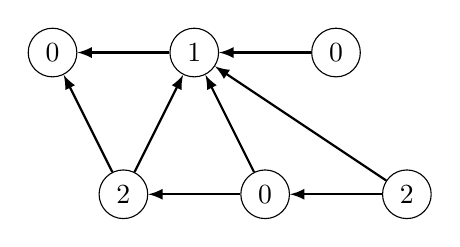
\begin{tikzpicture}[scale=0.9]
\node[draw, circle] (1) at (0,0) {0};
\node[draw, circle] (2) at (2,0) {1};
\node[draw, circle] (3) at (4,0) {0};
\node[draw, circle] (4) at (1,-2) {2};
\node[draw, circle] (5) at (3,-2) {0};
\node[draw, circle] (6) at (5,-2) {2};

\path[draw,thick,->,>=latex] (2) -- (1);
\path[draw,thick,->,>=latex] (3) -- (2);
\path[draw,thick,->,>=latex] (5) -- (4);
\path[draw,thick,->,>=latex] (6) -- (5);
\path[draw,thick,->,>=latex] (4) -- (1);
\path[draw,thick,->,>=latex] (4) -- (2);
\path[draw,thick,->,>=latex] (5) -- (2);
\path[draw,thick,->,>=latex] (6) -- (2);
\end{tikzpicture}
\end{center}
負けた状態のGrundy数は0で勝った状態のGrundy数は正の数です。

ある状態のGrundy数とは、nimの山のスティックの本数に相当します。
Grundy数が0であれば、グランディ数が正である状態にのみ移動でき、
Grundy数が$x > 0$であれば、Grundy数が$0,1,\ldots,x-1$のすべての数を含む状態に移動することが可能になります。

例として、迷路の中で図形を動かすゲームを考えます。
迷路の各マスは、床か壁のどちらかです。
手番で、プレイヤーは図形を左か上に何歩か移動させなければならないとします。
最後に動かしたプレイヤーが勝者です。

次の図は、ゲームの初期状態の例です。@は図形、*は移動可能なマスを表します。
\begin{center}
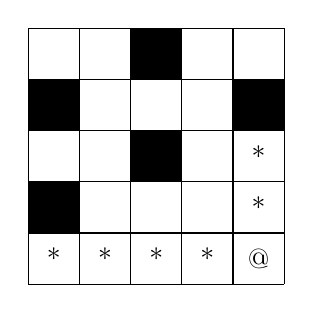
\begin{tikzpicture}[scale=.65]
  \begin{scope}
    \fill [color=black] (0, 1) rectangle (1, 2);
    \fill [color=black] (0, 3) rectangle (1, 4);
    \fill [color=black] (2, 2) rectangle (3, 3);
    \fill [color=black] (2, 4) rectangle (3, 5);
    \fill [color=black] (4, 3) rectangle (5, 4);

    \draw (0, 0) grid (5, 5);

    \node at (4.5,0.5) {@};
    \node at (3.5,0.5) {*};
    \node at (2.5,0.5) {*};
    \node at (1.5,0.5) {*};
    \node at (0.5,0.5) {*};
    \node at (4.5,1.5) {*};
    \node at (4.5,2.5) {*};

  \end{scope}
\end{tikzpicture}
\end{center}

ゲームの状態は、迷路のすべての床のマス目で表現できます。
上の迷路では、Grundy数は以下の通りです。


\begin{center}
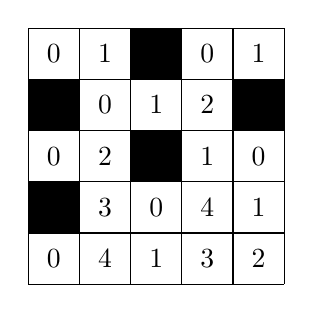
\begin{tikzpicture}[scale=.65]
  \begin{scope}
    \fill [color=black] (0, 1) rectangle (1, 2);
    \fill [color=black] (0, 3) rectangle (1, 4);
    \fill [color=black] (2, 2) rectangle (3, 3);
    \fill [color=black] (2, 4) rectangle (3, 5);
    \fill [color=black] (4, 3) rectangle (5, 4);

    \draw (0, 0) grid (5, 5);

    \node at (0.5,4.5) {0};
    \node at (1.5,4.5) {1};
    \node at (2.5,4.5) {};
    \node at (3.5,4.5) {0};
    \node at (4.5,4.5) {1};

    \node at (0.5,3.5) {};
    \node at (1.5,3.5) {0};
    \node at (2.5,3.5) {1};
    \node at (3.5,3.5) {2};
    \node at (4.5,3.5) {};

    \node at (0.5,2.5) {0};
    \node at (1.5,2.5) {2};
    \node at (2.5,2.5) {};
    \node at (3.5,2.5) {1};
    \node at (4.5,2.5) {0};

    \node at (0.5,1.5) {};
    \node at (1.5,1.5) {3};
    \node at (2.5,1.5) {0};
    \node at (3.5,1.5) {4};
    \node at (4.5,1.5) {1};

    \node at (0.5,0.5) {0};
    \node at (1.5,0.5) {4};
    \node at (2.5,0.5) {1};
    \node at (3.5,0.5) {3};
    \node at (4.5,0.5) {2};
  \end{scope}
\end{tikzpicture}
\end{center}

したがって、
迷路ゲームの各状態は、nimゲームの山に対応する。
例えば、右下のマスのGrundy数は2なので、
勝利状態です。
4歩左に移動するか、2歩上に移動するかで負け状態に遷移できるので、ゲームに勝つことができます。

なお、本来のnimゲームとは異なり、現在の状態のGrundy数よりも大きなGrundy数を持つ状態に移動も可能です。
ただし、相手はそれを打ち消す手を常に選べるので、負け状態から脱出することはできません。

\subsubsection{サブゲーム - Subgames}

次に、このゲームがサブゲームから構成されていると仮定します。
各ターンにおいて、プレイヤーはまずサブゲームを選択し、
次にサブゲームにおける一手を選択するものとしましょう。
ゲームは、どのサブゲームでも手を打つことができなくなったときに終了します。

この場合、複数のサブゲームから構成されるあるゲームのGrundy数は、
サブゲームのGrundy数のNim和となります。

サブゲームのGrundy数をすべて計算し、そのNim和を計算することで、
Nimゲームのようにプレイすることができます。

例として、3つの迷路のサブゲームで構成されるゲームを考えてみましょう。
このゲームでは、プレイヤーは手番ごとに迷路の一つを選び、その迷路の中で図形を移動させられるとします。
ゲームの初期状態を次のように仮定しましょう。
\begin{center}
\begin{tabular}{ccc}
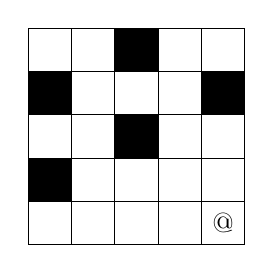
\begin{tikzpicture}[scale=.55]
  \begin{scope}
    \fill [color=black] (0, 1) rectangle (1, 2);
    \fill [color=black] (0, 3) rectangle (1, 4);
    \fill [color=black] (2, 2) rectangle (3, 3);
    \fill [color=black] (2, 4) rectangle (3, 5);
    \fill [color=black] (4, 3) rectangle (5, 4);

    \draw (0, 0) grid (5, 5);

    \node at (4.5,0.5) {@};

    \end{scope}
\end{tikzpicture}
&
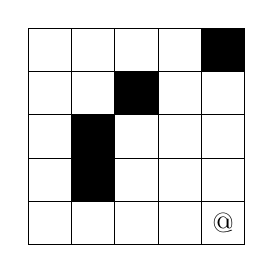
\begin{tikzpicture}[scale=.55]
  \begin{scope}
    \fill [color=black] (1, 1) rectangle (2, 3);
    \fill [color=black] (2, 3) rectangle (3, 4);
    \fill [color=black] (4, 4) rectangle (5, 5);

    \draw (0, 0) grid (5, 5);

    \node at (4.5,0.5) {@};

  \end{scope}
\end{tikzpicture}
&
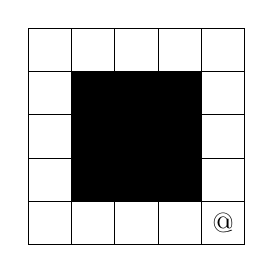
\begin{tikzpicture}[scale=.55]
  \begin{scope}
    \fill [color=black] (1, 1) rectangle (4, 4);

    \draw (0, 0) grid (5, 5);

    \node at (4.5,0.5) {@};
  \end{scope}
\end{tikzpicture}
\end{tabular}
\end{center}

各迷路に置けるGrundy数は以下の通りになります。

\begin{center}
\begin{tabular}{ccc}
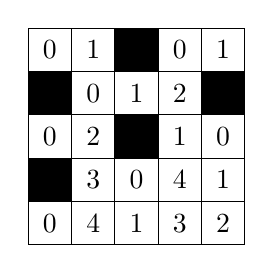
\begin{tikzpicture}[scale=.55]
  \begin{scope}
    \fill [color=black] (0, 1) rectangle (1, 2);
    \fill [color=black] (0, 3) rectangle (1, 4);
    \fill [color=black] (2, 2) rectangle (3, 3);
    \fill [color=black] (2, 4) rectangle (3, 5);
    \fill [color=black] (4, 3) rectangle (5, 4);

    \draw (0, 0) grid (5, 5);

    \node at (0.5,4.5) {0};
    \node at (1.5,4.5) {1};
    \node at (2.5,4.5) {};
    \node at (3.5,4.5) {0};
    \node at (4.5,4.5) {1};

    \node at (0.5,3.5) {};
    \node at (1.5,3.5) {0};
    \node at (2.5,3.5) {1};
    \node at (3.5,3.5) {2};
    \node at (4.5,3.5) {};

    \node at (0.5,2.5) {0};
    \node at (1.5,2.5) {2};
    \node at (2.5,2.5) {};
    \node at (3.5,2.5) {1};
    \node at (4.5,2.5) {0};

    \node at (0.5,1.5) {};
    \node at (1.5,1.5) {3};
    \node at (2.5,1.5) {0};
    \node at (3.5,1.5) {4};
    \node at (4.5,1.5) {1};

    \node at (0.5,0.5) {0};
    \node at (1.5,0.5) {4};
    \node at (2.5,0.5) {1};
    \node at (3.5,0.5) {3};
    \node at (4.5,0.5) {2};
    \end{scope}
\end{tikzpicture}
&
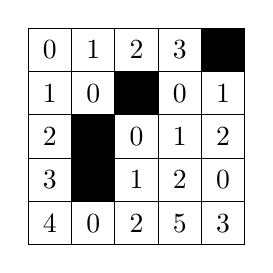
\begin{tikzpicture}[scale=.55]
  \begin{scope}
    \fill [color=black] (1, 1) rectangle (2, 3);
    \fill [color=black] (2, 3) rectangle (3, 4);
    \fill [color=black] (4, 4) rectangle (5, 5);

    \draw (0, 0) grid (5, 5);

    \node at (0.5,4.5) {0};
    \node at (1.5,4.5) {1};
    \node at (2.5,4.5) {2};
    \node at (3.5,4.5) {3};
    \node at (4.5,4.5) {};

    \node at (0.5,3.5) {1};
    \node at (1.5,3.5) {0};
    \node at (2.5,3.5) {};
    \node at (3.5,3.5) {0};
    \node at (4.5,3.5) {1};

    \node at (0.5,2.5) {2};
    \node at (1.5,2.5) {};
    \node at (2.5,2.5) {0};
    \node at (3.5,2.5) {1};
    \node at (4.5,2.5) {2};

    \node at (0.5,1.5) {3};
    \node at (1.5,1.5) {};
    \node at (2.5,1.5) {1};
    \node at (3.5,1.5) {2};
    \node at (4.5,1.5) {0};

    \node at (0.5,0.5) {4};
    \node at (1.5,0.5) {0};
    \node at (2.5,0.5) {2};
    \node at (3.5,0.5) {5};
    \node at (4.5,0.5) {3};
  \end{scope}
\end{tikzpicture}
&
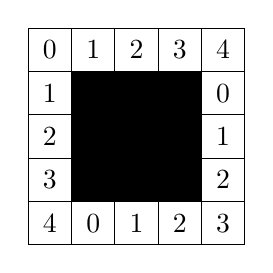
\begin{tikzpicture}[scale=.55]
  \begin{scope}
    \fill [color=black] (1, 1) rectangle (4, 4);

    \draw (0, 0) grid (5, 5);

    \node at (0.5,4.5) {0};
    \node at (1.5,4.5) {1};
    \node at (2.5,4.5) {2};
    \node at (3.5,4.5) {3};
    \node at (4.5,4.5) {4};

    \node at (0.5,3.5) {1};
    \node at (1.5,3.5) {};
    \node at (2.5,3.5) {};
    \node at (3.5,3.5) {};
    \node at (4.5,3.5) {0};

    \node at (0.5,2.5) {2};
    \node at (1.5,2.5) {};
    \node at (2.5,2.5) {};
    \node at (3.5,2.5) {};
    \node at (4.5,2.5) {1};

    \node at (0.5,1.5) {3};
    \node at (1.5,1.5) {};
    \node at (2.5,1.5) {};
    \node at (3.5,1.5) {};
    \node at (4.5,1.5) {2};

    \node at (0.5,0.5) {4};
    \node at (1.5,0.5) {0};
    \node at (2.5,0.5) {1};
    \node at (3.5,0.5) {2};
    \node at (4.5,0.5) {3};
  \end{scope}
\end{tikzpicture}
\end{tabular}
\end{center}

初期状態が$2 \oplus 3 \oplus 3 = 2$
であるため、先攻が勝利します。
例えば、最初の1手で2マス上に進めば、$0 \oplus 3 \oplus 3 = 0$を生成して相手に渡せます。

\subsubsection{Grundyゲーム - Grundy's game}

ある対局の一手が、
その対局を互いに独立した下位の対局に分割するとみなせることがあります。
この場合、そのゲームのGrundy数は
\[\textrm{mex}(\{g_1, g_2, \ldots, g_n \}),\]
となり、$n$はゲームの可能な手の数です。
\[g_k = a_{k,1} \oplus a_{k,2} \oplus \ldots \oplus a_{k,m},\]
$k$の手順は$a_{k,1},a_{k,2},\ldots,a_{k,m}$のサブゲームを生成するとします。

\index{Grundyゲーム - Grundy's game}

\key{Grundyゲーム - Grundy's game}はこのようなゲームの例です。
初期状態では、$n$本の棒を含む一つの山があります。
手番ごとに,プレイヤーは山を選び,それを空でない二つの山に分割し,
その山の大きさが異なるようにしなければなりません。最後に手を打ったプレイヤーがゲームに勝ちます。

$n$本の棒を含むヒープのGrundy数を$f (n)$としましょう。
Grundy数は、
山を2つの山に分割する方法をすべて調べれば計算できます。
例えば,$n = 8$のとき$1+7$, $2+6$ , $3+5$の可能性があるので以下のようになります。
\[f(8)=\textrm{mex}(\{f(1) \oplus f(7), f(2) \oplus f(6), f(3) \oplus f(5)\}).\]

このゲームでは,$f (n)$ の値は,$f(1),\ldots,f(n-1)$の値に基づいて決定されます。
1本と2本の棒の山を分割することはできないので$f(1)=f(2)=0$であることに注意します。
\[
\begin{array}{lcl}
f(1) & = & 0 \\
f(2) & = & 0 \\
f(3) & = & 1 \\
f(4) & = & 0 \\
f(5) & = & 2 \\
f(6) & = & 1 \\
f(7) & = & 0 \\
f(8) & = & 2 \\
\end{array}
\]
$n=8$のときのグランディ数は2なので、ゲームに勝つことは可能です。
$f(1) \oplus f(7) = 0$なので、勝ち手はヒープ$1+7$を作ることです。